\subsection{Немного о бифуркациях.}
Будем рассматривать параметрические динамические системы вида
\[
    \dot{\bt{x}} = \bt{f}(\bt{x}, \bt{\alpha}).
\]
Равновесия этих систем ищутся из уравнения $\bt{f}(\bt{x}, \bt{\alpha}) = 0$ (естественно, относительно переменных $\bt{x}$).
\begin{example}
    Рассмотрим одномерную динамическую систему вида
    \[
        \dot{x} = x^2 + \alpha.
    \]
    Её равновесиями являются $x^* = \pm\sqrt{-\alpha}$.
    При $\alpha < 0$ есть два положения равновесия: $\pm \sqrt {-\alpha}$.
    Из них $-\sqrt {-\alpha}$ является устойчивым, поскольку фазовый поток сходится к нему, а второе -- неустойчивое.
    При $\alpha = 0$ есть только нулевое положение равновесия и оно не является устойчивым.
    При положительных $\alpha$ положений равновесия нет в принципе.
    \begin{figure*}[h!]
        \centering
        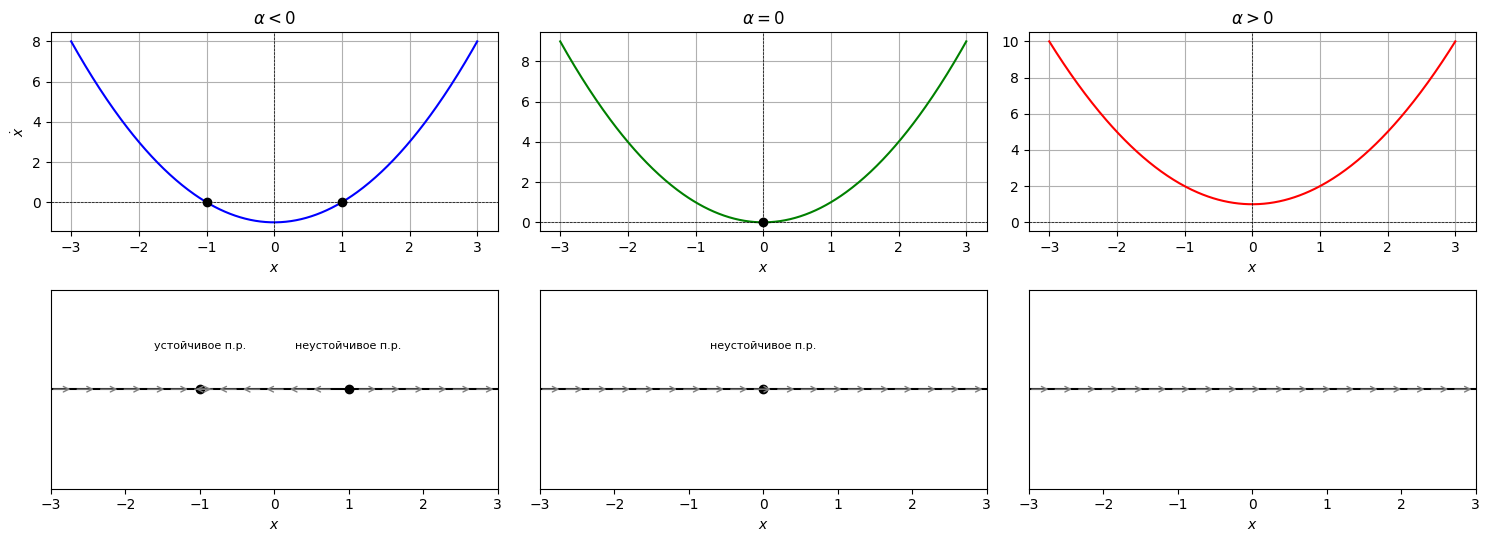
\includegraphics[width=1\linewidth]{images/simplebifurcation}
        \caption{Линейные фазовые диаграммы и положения равновесия для $\dot{x} = x^2 + \alpha$.}
    \end{figure*} \\
    Заметим, что при переходе $\alpha$ через ноль у нас изменяется число положений равновесия и их характеристики.
    Подобные <<изменения>> называются бифуркациями.
    Для них принято рисовать диаграммы подобного \hyperref[fig:simple_bif_diag]{вида}
    \begin{figure*}[h!]
        \centering
        \label{fig:simple_bif_diag}
        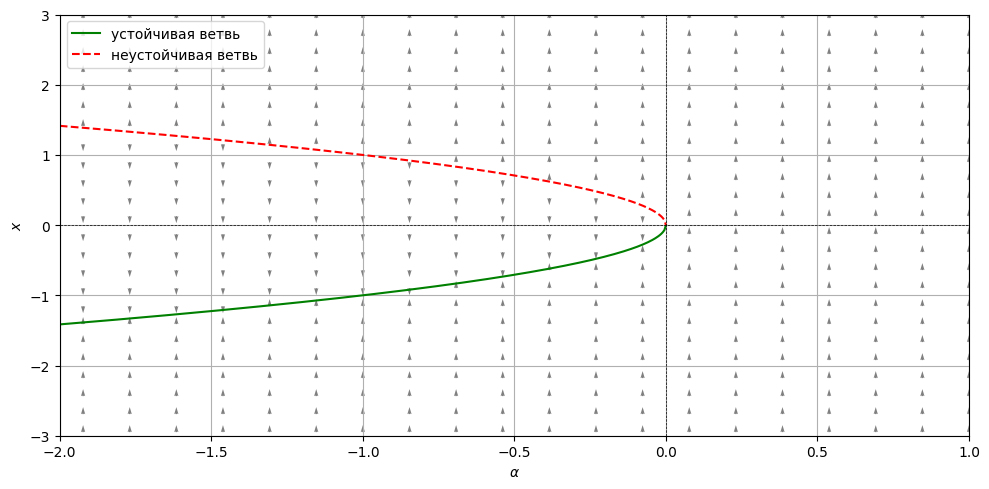
\includegraphics[width=0.8\linewidth]{images/simplebifurcationdiagramm}
        \caption{Бифуркационная диаграмма для $\dot{x} = x^2 + \alpha$.}
    \end{figure*} \\
    Видно, что $\alpha = 0$ -- особая точка.
    Более формально, $\forall \alpha$ по теореме о неявной функции $\exists!$ решение $x(\alpha) = x^*$ если $\dfrac{\partial f}{\partial x} \neq 0$.
    Соответственно, будем называть бифуркацией положение равновесия, в котором это не выполняется: $f(x, \alpha) = 0$ и $\dfrac{\partial f}{\partial x} = 0$.
    Для нашей системы это
    \[
        \begin{cases}
            x^2 + \alpha = 0 \\
            2x = 0
        \end{cases} \Ra \begin{cases}
                            x = 0 \\
                            \alpha = 0
        \end{cases}
    \]
    Подобный тип бифуркаций называется <<седло-узел>>.
\end{example}
\begin{example}[Пример бифуркации типа <<смена устойчивости>>]
    Рассмотрим динамическую систему вида 
    \[
        \dot{x} = \alpha x - x^2.
    \]
    У нас всегда есть две равновесные кривые: $x = 0$ и $x = \alpha$.
    При этом, точка $x = 0, \alpha = 0$ -- особая и там происходит бифуркация вида <<смена устойчивости>>.
    Она выглядит как на \hyperref[fig:transcritical_diag]{вот этом графике}.
    \begin{figure*}[h!]
        \centering
        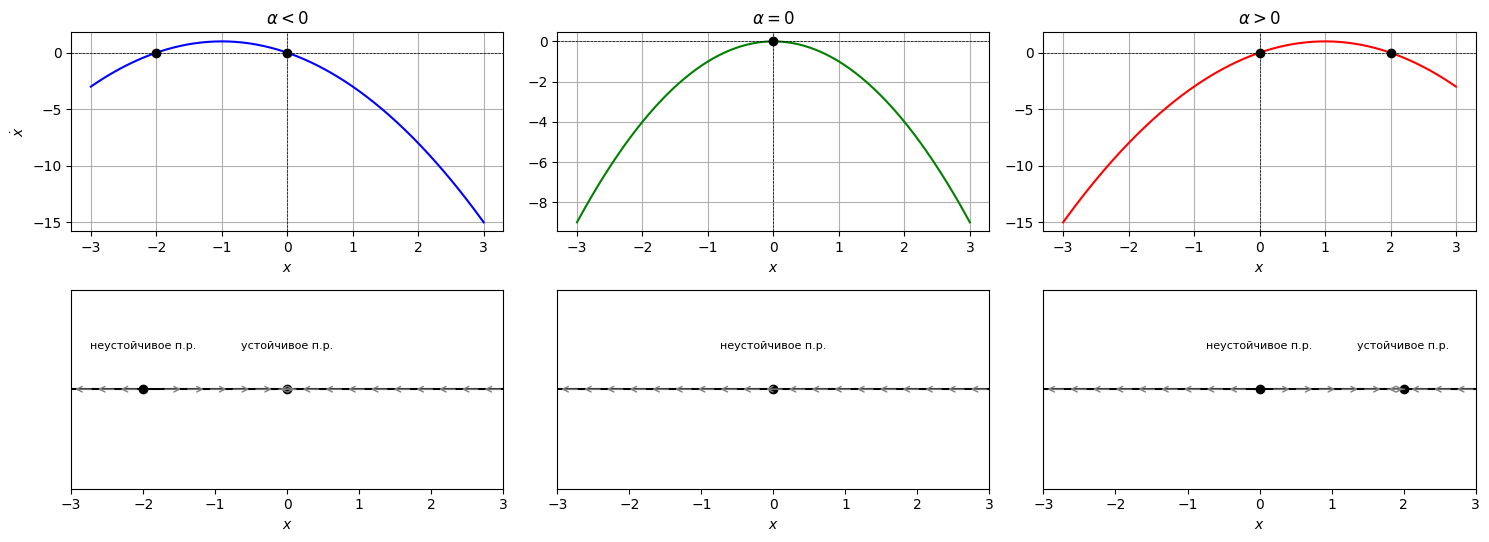
\includegraphics[width=1\linewidth]{images/transcritical_phase}
        \caption{Линейные фазовые диаграммы и положения равновесия для $\dot{x} = \alpha x - x^2$.}
    \end{figure*}
    \begin{figure*}[h!]
        \centering
        \label{fig:transcritical_diag}
        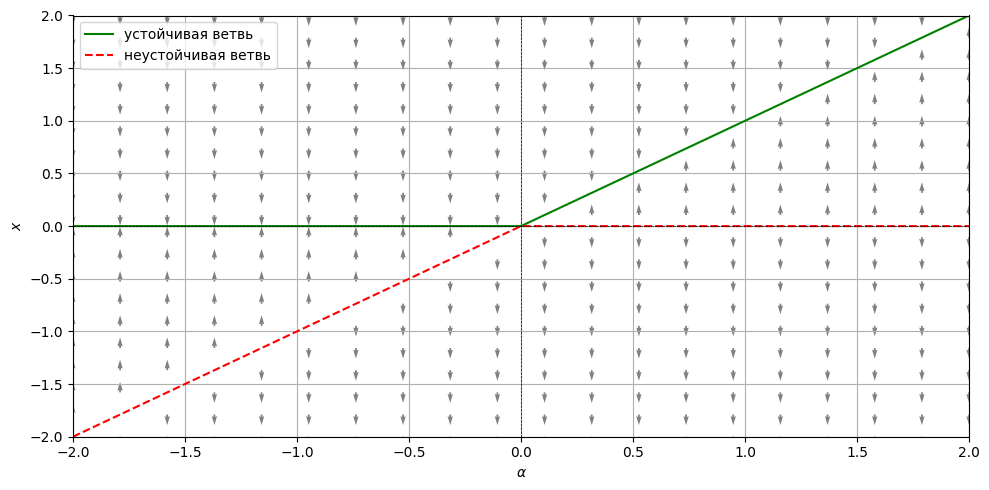
\includegraphics[width=0.8\linewidth]{images/transcritical_diagram}
        \caption{Бифуркационная диаграмма для $\dot{x} = \alpha x - x^2$.}
    \end{figure*}
\end{example}
\begin{example}[Пример бифуркации типа <<вилка>>]
    Теперь рассмотрим ДУ вида
    \[
        \dot{x} = \alpha x - x^3.
    \]
    При неположительных $\alpha$ имеется ровно одно положение равновесие -- нулевое, и оно является устойчивым.
    При переходе через ноль происходит бифуркация типа <<вилка>> и добавляются две устойчивые ветви $\pm \sqrt {\alpha}$, а $x = 0$ становится неустойчивым.
    Бифуркационная диаграмма выглядит примерно \hyperref[fig:pitchfork_diag]{так}.
    \begin{figure*}[h!]
        \centering
        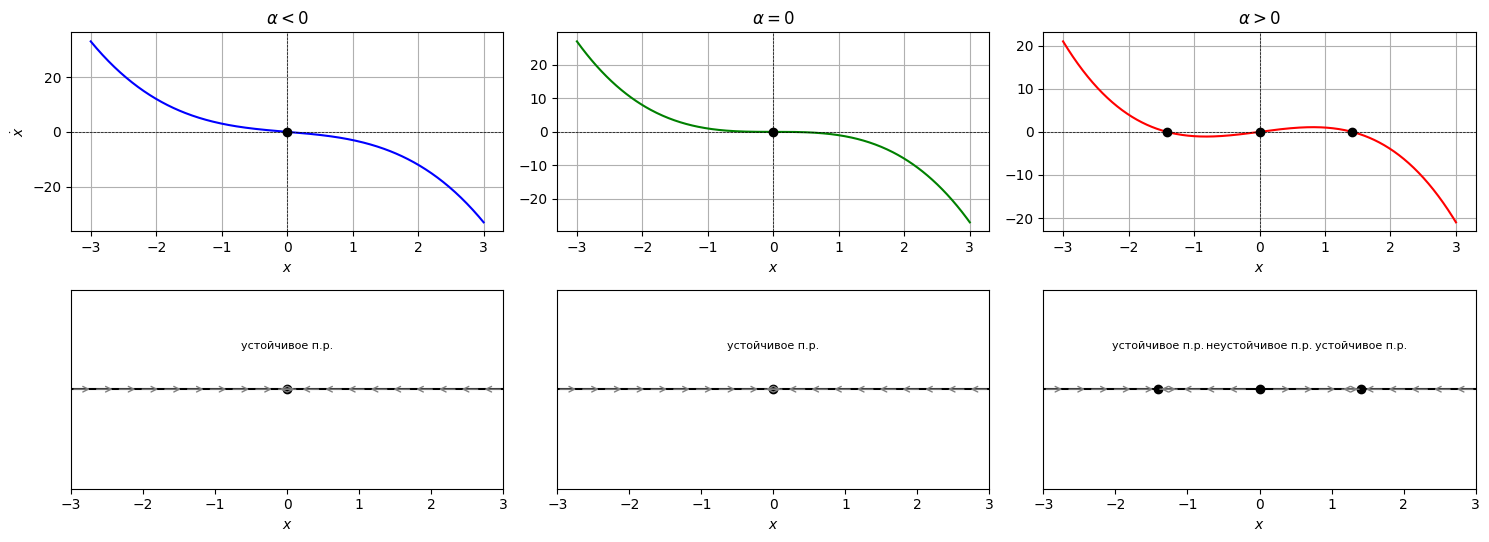
\includegraphics[width=1\linewidth]{images/pitchfork_phase}
        \caption{Линейные фазовые диаграммы и положения равновесия для $\dot{x} = \alpha x - x^3$.}
    \end{figure*}
    \begin{figure*}[h!]
        \centering
        \label{fig:pitchfork_diag}
        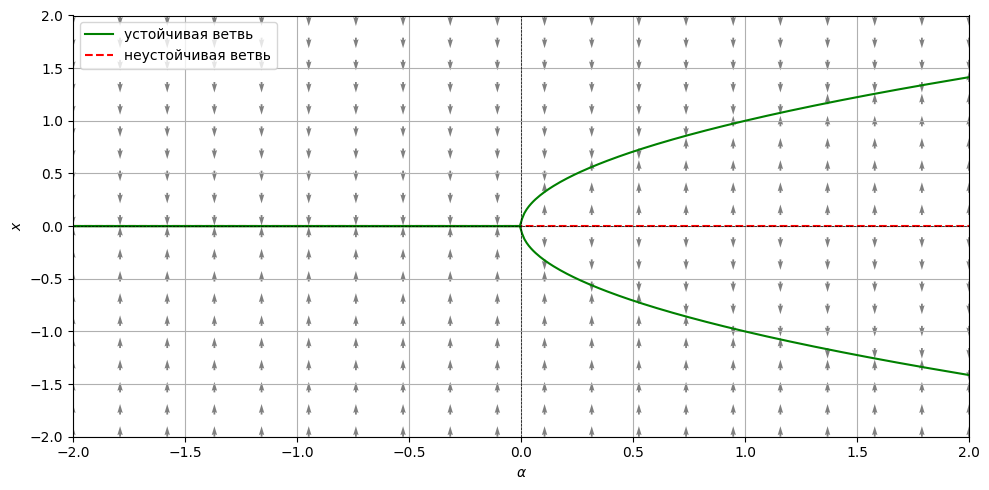
\includegraphics[width=0.8\linewidth]{images/pitchfork_diagram}
        \caption{Бифуркационная диаграмма для $\dot{x} = \alpha x - x^3$.}
    \end{figure*}
\end{example}
\begin{example}[Явление гистерезиса]
    Рассмотрим систему вида
    \[
        \dot{x} = \alpha - x^3 + x.
    \]
    Её положения равновесия определяются из уравнения $\alpha = x^3 - x$, и эта система имеет гистерезис, как можно увидеть по \hyperref[fig:gisteresis_diag]{бифуркационной диаграмме}.
    \begin{center}
        \begin{figure*}[h!]
            \centering
            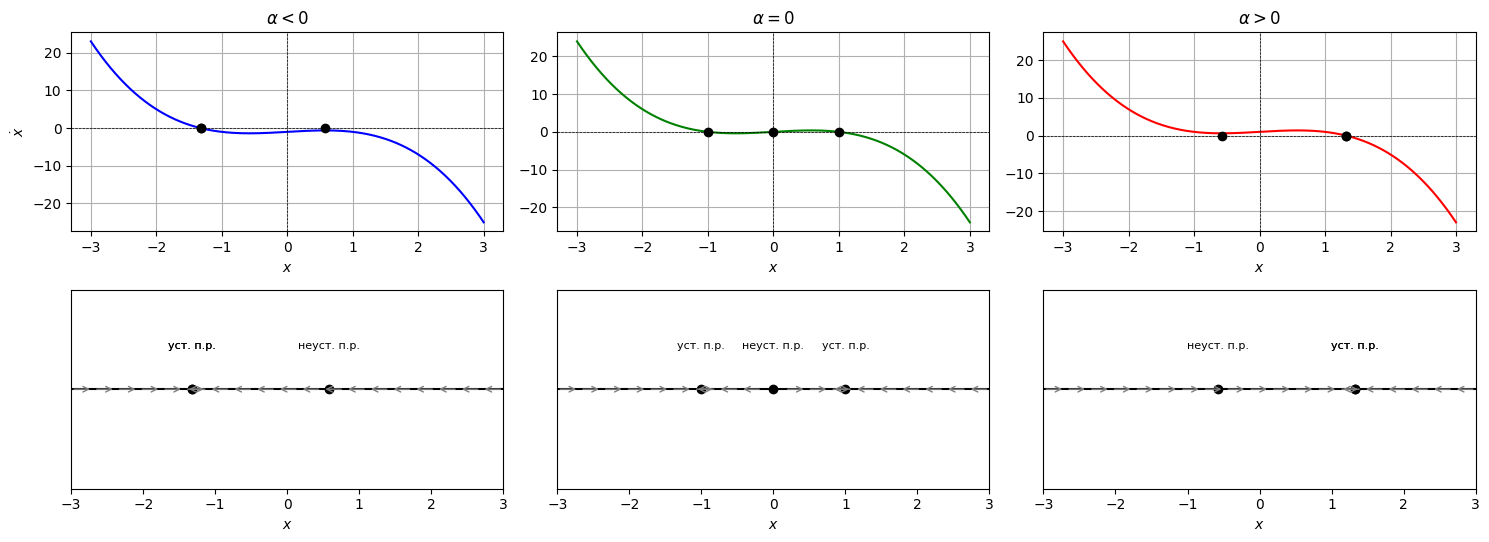
\includegraphics[width=1\linewidth]{images/gisteresis_phase}
            \caption{Линейные фазовые диаграммы и положения равновесия для $\dot{x} = \alpha - x^3 + x$.}
        \end{figure*}
        \begin{figure*}[h!]
            \centering
            \label{fig:gisteresis_diag}
            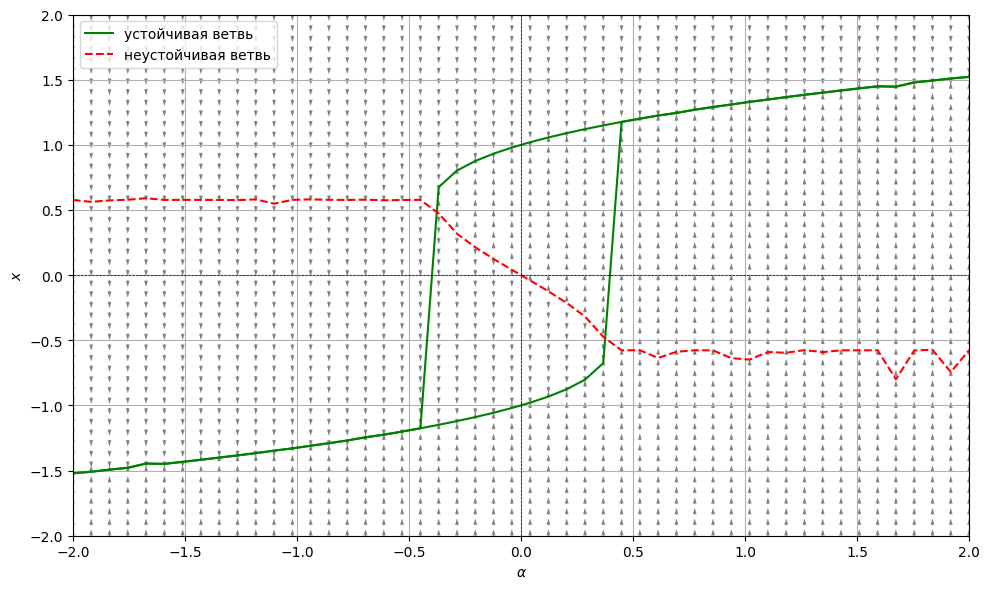
\includegraphics[width=0.8\linewidth]{images/gisteresis_diagram}
            \caption{Бифуркационная диаграмма для $\dot{x} = \alpha - x^3 + x$.}
        \end{figure*}
    \end{center}
\end{example}
\begin{note}[Примечание техающего]
    Более подробно можно почитать в пособии в разделе <<учебные пособия>> кафедры теоретической механики на сайте фт.
\end{note}
Но вот это всё было про одномерные системы.
В многомерных системах могут быть не только бифуркации, но и такие сущности как предельные циклы и аттракторы.
\begin{definition}
    Предельным циклом будем называть замкнутую периодическую траекторию решения динамической системы такую, что
    \begin{itemize}
        \item В некоторой окрестности цикла нет других периодических траекторий
        \item Все траектории в этой окрестности сходятся к предельному циклу при $t \ra \infty$ (или при $t \ra -\infty$)
    \end{itemize}
    Будем называть предельный цикл устойчивым, если траектории в окрестности сходятся к нему при $t \ra +\infty$ и неустойчивым если при $t \ra -\infty$.
    Если же существуют как траектории одного вида, так и траектории другого вида, то будем называть такой цикл полуустойчивым.
\end{definition}
\begin{example}[Пример устойчивого предельного цикла: осциллятор Ван-дер-Поля.]
    Рассмотрим следующую двумерную динамическую систему:
    \begin{equation*}
        \begin{cases}
            \dot{x} = y \\
            \dot{y} = \mu(1 - x^2)y - x.
        \end{cases}
    \end{equation*}
    Она называется <<осциллятором Ван-дер-Поля>> и обладает устойчивым предельным циклом при $\mu > 0$ следующего \hyperref[fig:van_der_pole_stable]{вида}.
    \begin{figure*}[h!]
        \centering
        \label{fig:van_der_pole_stable}
        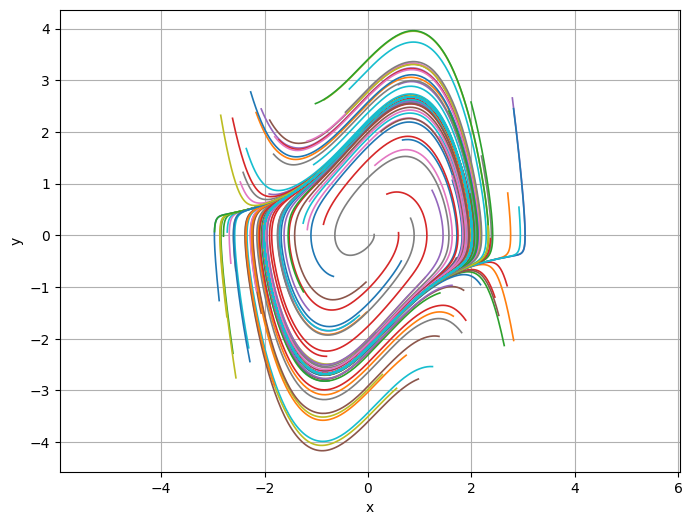
\includegraphics[width=0.8\linewidth]{images/vanderpole_stable}
        \caption{Предельный цикл осциллятора Ван-дер-Поля.}
    \end{figure*}
\end{example}
\begin{definition}
    Аттрактором динамической системы называется такое компактное подмножество евклидового пространства, что к нему стремятся все решения динамической системы с начальными условиями в некоторой области.
    Сама область (или объединение некоторого их количества) называется бассейном аттрактора.
\end{definition}
\begin{example}[Аттрактор Лоренца]
    В системе, задающейся уравнениями
    \[
        \begin{cases}
            \dot{x} = \sigma(y - x)\\
            \dot{y} = x(r - z) - y\\
            \dot{z} = xy - bz.
        \end{cases}
    \]
    Существует аттрактор следующего \hyperref[fig:lorentz_attractor]{вида}.
    \begin{figure*}[h!]
        \centering
        \label{fig:lorentz_attractor}
        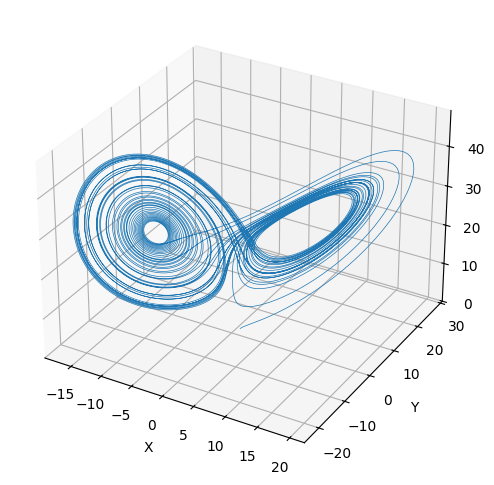
\includegraphics[width=0.8\linewidth]{images/lorentz_attractor}
        \caption{<<Странный аттрактор>> Лоренца.}
    \end{figure*}
\end{example}
\begin{example}
    В динамических системах старших размерностей встречаются новые виды бифуркаций.
    В частности, бифуркация рождения предельного цикла Андронова-Хопфа.
    Примером простейшей системы в которой она возникает служит
    \[
        \begin{cases}
            \dot{x} = \alpha x - y - x(x^2 + y^2) \\
            \dot{y} = x + \alpha y - y(x^2 + y^2).
        \end{cases}
    \]
    Точкой бифуркации является ноль (нетрудно заметить что независимо от $\alpha$ ноль всегда является положением равновесия).
    В линейном приближении матрицей системы является
    \[
        A = \begin{pmatrix*} \alpha & -1 \\ 1 & \alpha.
        \end{pmatrix*}
    \]
    собственные значения которой равны $\alpha \pm i$.
    Таким образом, при $\alpha < 0$ положение равновесия является устойчивым, а при $\alpha > 0$ -- неустойчивым.
    Перейдём к полярным координатам:
    \[
        \begin{cases}
            x = r \cos \phi \\
            y =  r \sin \phi.
        \end{cases}
    \]
    Путём несложных преобразований мы получаем систему следующего вида:
    \[
        \begin{cases}
            \dot{r} = r(\alpha - r^2) \\
            \dot{\phi} = 1.
        \end{cases}
    \]
    При положительных $\alpha$ уравнение по $r$ имеет два положения равновесия: $r = 0$ и $r = \sqrt {\alpha}$.
    Ранее показано что нулевое равновесие неустойчиво.
    Второе положение равновесия является асимптотически устойчивым (опять-таки, это можно показать с использованием линейного приближения).
    В силу отделённости $r$ и $\phi$ у нас получается устойчивый предельный цикл, который выглядит следующим \hyperref[fig:hopf_bifurcation]{образом}.
    \begin{figure*}[ht!]
        \centering
        \label{fig:hopf_bifurcation}
        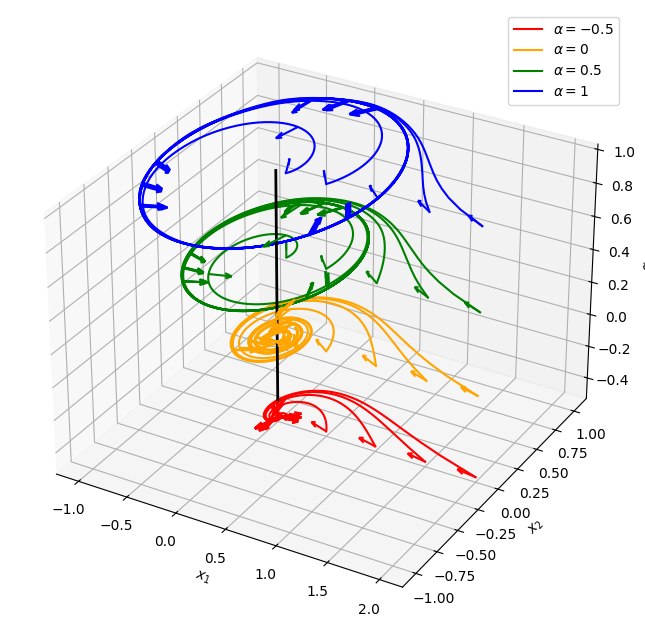
\includegraphics[width=0.8\linewidth]{images/hopf_bifurcation}
        \caption{Рождение предельного цикла.}
    \end{figure*}
\end{example}
\begin{definition}
    Потеря устойчивости, происходящая при бифуркации Андронова-Хопфа называется мягкой (а сам эффект называется флаттером).
\end{definition}
\begin{definition}
    Потеря устойчивости, происходящая при исчезновении равновесия в бифуркации типа складки называется жёсткой (а сам эффект -- дивергенцией).
\end{definition}
% Пример дивергенции.
% Логистическое отображение и динамический хаос.